\documentclass [12pt ,a4paper, english]{scrartcl}

\usepackage []{inputenc}
\usepackage [english]{babel}
\usepackage {lmodern}
\usepackage [T1]{fontenc}

\usepackage {fancyhdr}
\usepackage {varioref}
\usepackage[colorlinks=true,linkcolor=black]{hyperref}


\usepackage {amsmath}
\usepackage {amssymb}
\usepackage {amsthm}
\usepackage {parskip}

\usepackage{xcolor}
\usepackage[pdftex]{graphicx}

\usepackage{listings}
\usepackage{color}

\definecolor{dkgreen}{rgb}{0,0.6,0}
\definecolor{gray}{rgb}{0.5,0.5,0.5}
\definecolor{mauve}{rgb}{0.58,0,0.82}

{
\lstset{frame=tb,
  language=Java,
  aboveskip=3mm,
  belowskip=3mm,
  showstringspaces=false,
  columns=flexible,
  basicstyle={\small\ttfamily},
  numbers=none,
  numberstyle=\tiny\color{gray},
  keywordstyle=\color{blue},
  commentstyle=\color{dkgreen},
  stringstyle=\color{mauve},
  breaklines=true,
  breakatwhitespace=true,
  tabsize=2,
  showspaces=false,
  showtabs=false,
}

\DeclareMathOperator{\spn}{span}

\theoremstyle{plain}
\newtheorem{thm}{Theorem}[section]
\newtheorem{lem}[thm]{Lemma}
\newtheorem{prop}[thm]{Proposition}

\theoremstyle{definition}
\newtheorem{defn}[thm]{Definition}
\newtheorem{conj}[thm]{Vermutung}
\newtheorem{bsp}[thm]{Beispiel}
\newtheorem{bem}[thm]{Remark}

\theoremstyle{remark}
\newtheorem*{note}{Notiz}
\newtheorem{case}{Case}

\author{Christoph Hofer\\ 0955139 \and Stefan Lew \\ 0856722}

\title{Mitzi - Exercise 3}
\fancyhf{}
\pagestyle {fancy}
\lhead {\textsc {\nouppercase{\leftmark}}}
\setlength\headheight{15pt}
\lfoot {Christoph Hofer, Stefan Lew}
\rfoot {Seite \thepage}
\renewcommand{\footrulewidth}{0.5 pt}
\renewcommand{\headheight}{29 pt}

\begin{document}
\maketitle
\newpage
\tableofcontents
\newpage

\section{Output of GUI}
The GIU uses the Java swing library. A 8$\times$8 grid is created and on every square a label represents the piece. When the program is started you can choose who should start, you or mitzi.
\begin{figure}[h!]
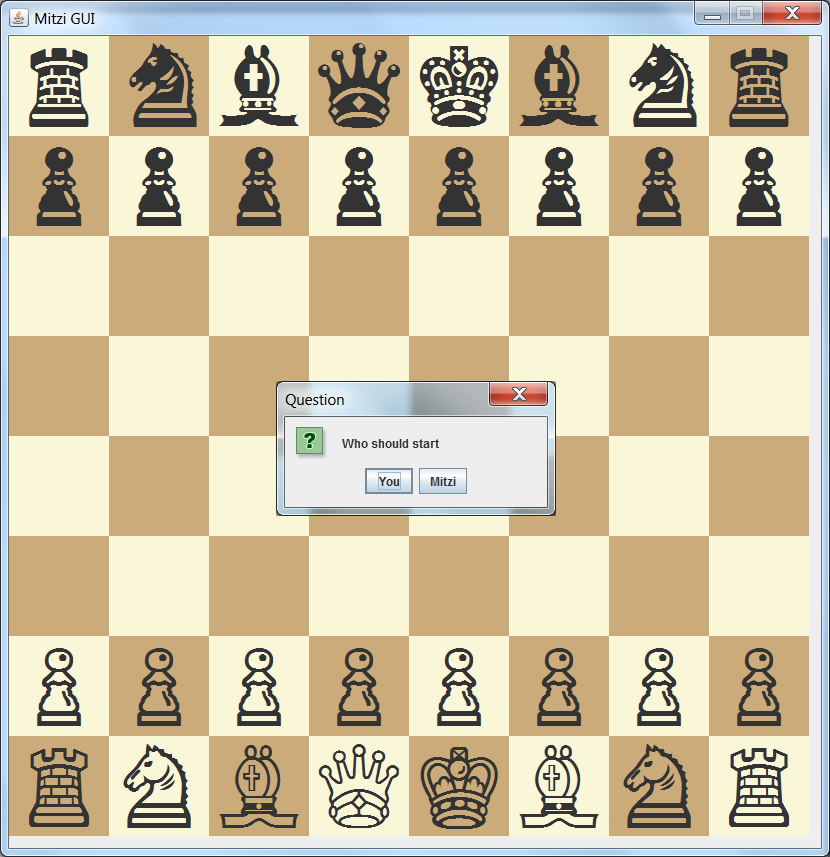
\includegraphics[scale=0.6]{out1.png}
\caption{Windows when you start the program}
\end{figure}

If its mitzis turn you are not able to move any piece and its checked that you can do only possible moves. After a move the whole board is redrawn using the fen string of the new position.

\begin{figure}[h!]
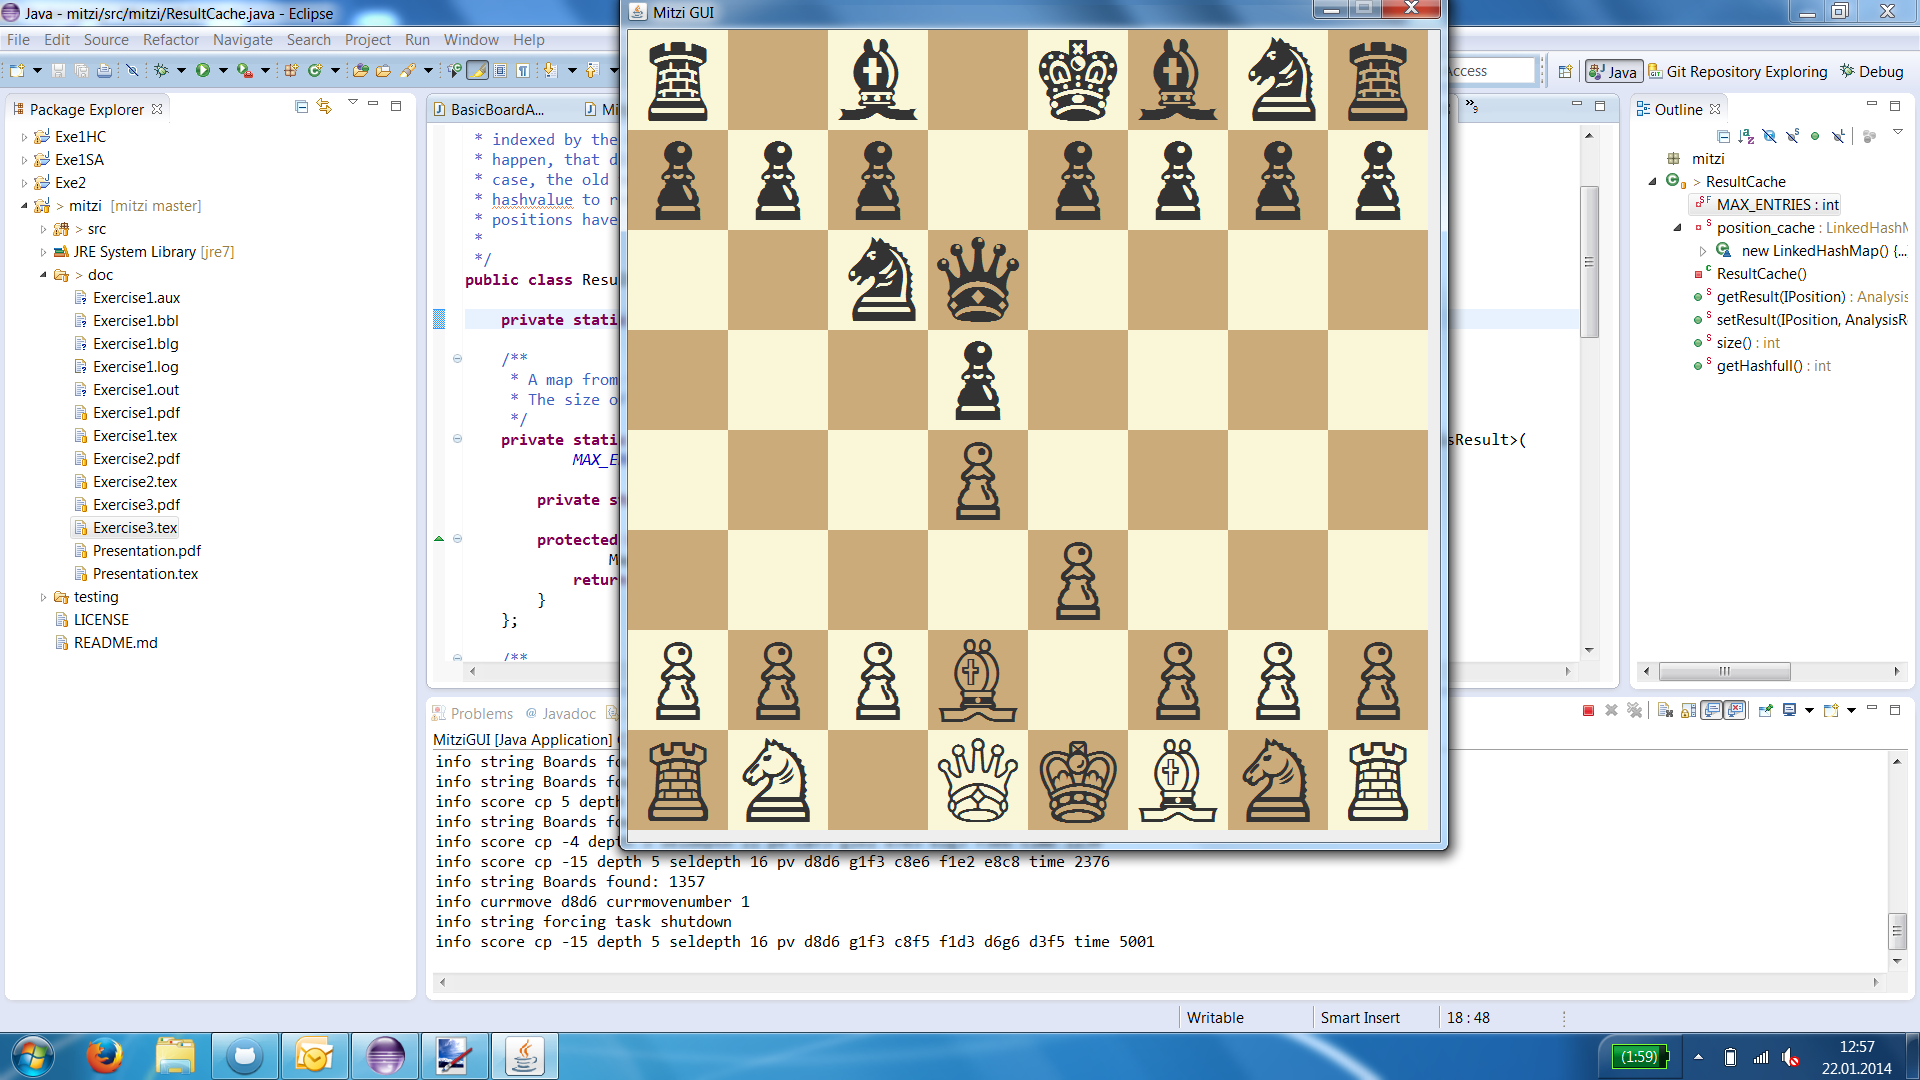
\includegraphics[scale=0.3]{out2.png}
\caption{Board after a view plys; you see in the background that mitzi is calculating.}
\end{figure}

\section{Our Final Code}

%\subsection{ChessGame.java}
%\lstinputlisting{../src/mitzi/ChessGame.java}

\subsection{Piece.java}
\lstinputlisting{../src/mitzi/Piece.java}

\subsection{Side.java}
\lstinputlisting{../src/mitzi/Side.java}

\subsection{PieceHelper.java}
\lstinputlisting{../src/mitzi/PieceHelper.java}

\subsection{SquareHelper.java}
\lstinputlisting{../src/mitzi/SquareHelper.java}

\subsection{IBrain.java}
\lstinputlisting{../src/mitzi/IBrain.java}

\subsection{IMove.java}
\lstinputlisting{../src/mitzi/IMove.java}

\subsection{IPosition.java}
\lstinputlisting{../src/mitzi/IPosition.java}

\subsection{IPositionAnalyzer.java}
\lstinputlisting{../src/mitzi/IPositionAnalyzer.java}
%
%\subsection{RandyBrain.java}
%\lstinputlisting{../src/mitzi/RandyBrain.java}
%
%\subsection{HumanBrain.java}
%\lstinputlisting{../src/mitzi/HumanBrain.java}

\subsection{Move.java}
\lstinputlisting{../src/mitzi/Move.java}

\subsection{Direction.java}
\lstinputlisting{../src/mitzi/Direction.java}

\subsection{Position.java}
\lstinputlisting{../src/mitzi/Position.java}

\subsection{AnalysisResult.java}
\lstinputlisting{../src/mitzi/AnalysisResult.java}

\subsection{BasicMoveComparator.java}
\lstinputlisting{../src/mitzi/BasicMoveComparator.java}

\subsection{CaptureComparator.java}
\lstinputlisting{../src/mitzi/CaptureComparator.java}
%
%\subsection{BasicBoardAnalyzer.java}
%\lstinputlisting{../src/mitzi/BasicBoardAnalyzer.java}

\subsection{BoardAnalyzer.java}
\lstinputlisting{../src/mitzi/BoardAnalyzer.java}

\subsection{Flag.java}
\lstinputlisting{../src/mitzi/Flag.java}

\subsection{GameState.java}
\lstinputlisting{../src/mitzi/GameState.java}

\subsection{IrreversibleMoveStack.java}
\lstinputlisting{../src/mitzi/IrreversibleMoveStack.java}

\subsection{KillerMoves.java}
\lstinputlisting{../src/mitzi/KillerMoves.java}

\subsection{MateScores.java}
\lstinputlisting{../src/mitzi/MateScores.java}

\subsection{MitziBrain.java}
\lstinputlisting{../src/mitzi/MitziBrain.java}

\subsection{ResultCache.java}
\lstinputlisting{../src/mitzi/ResultCache.java}

\subsection{UCIReporter.java}
\lstinputlisting{../src/mitzi/UCIReporter.java}

\subsection{MitziGUI.java}
\lstinputlisting{../src/mitzi/MitziGUI.java}

\end{document}
